\documentclass[10pt,twocolumn,letterpaper]{article}

\usepackage{cvpr}
\usepackage{times}
\usepackage{epsfig}
\usepackage{graphicx}
\usepackage{amsmath}
\usepackage{amssymb}

% Include other packages here, before hyperref.

% If you comment hyperref and then uncomment it, you should delete
% egpaper.aux before re-running latex.  (Or just hit 'q' on the first latex
% run, let it finish, and you should be clear).
\usepackage[breaklinks=true,bookmarks=false]{hyperref}

\cvprfinalcopy

% \def\cvprPaperID{****} % *** Enter the CVPR Paper ID here
\def\httilde{\mbox{\tt\raisebox{-.5ex}{\symbol{126}}}}

% Pages are numbered in submission mode, and unnumbered in camera-ready
%\ifcvprfinal\pagestyle{empty}\fi
\setcounter{page}{4321}
\begin{document}

%%%%%%%%% TITLE
\title{cDCGAN: conditional Deep Convolutional Generative Adversarial Networks}

\author{Edoardo De Matteis\\
La Sapienza University of Rome\\
{\tt\small dematteis.1746561@studenti.uniroma1.it}
}

\maketitle
%\thispagestyle{empty}

%%%%%%%%% ABSTRACT
\begin{abstract}
   GANs have been described as one of the most interesting idea in the last years of machine learning, and have been integrated with CNNs to have strong priors on images.
   Conditional GANs allow us to condition generation through supplementary input, in this project.
   I combine both these models in a conditional deep convolutional GAN, code is available at \href{https://github.com/edodema/cDCGAN}{https://github.com/edodema/cDCGAN}.
\end{abstract}

\section{Introduction}
Since they were first introduced in 2014 GANs have changed the game ~\cite{goodfellow2014generative}, to the point that Yann LeCun considers them the most interesting idea in the last 10 years of machine learning ~\cite{lecun2016riseminar}.
Their ability to generate realistic images has amazed both specialists and the general publi, e.g. the website \textit{This Person Does Not Exist} ()\href{https://thispersondoesnotexist.com/}{https://thispersondoesnotexist.com/}) based on \textit{StyleGAN2} ~\cite{viazovetskyi2020stylegan2}.
StyleGAN2 has been recently overcome by \textit{StyleGAN3} ~\cite{DBLP:journals/corr/abs-2106-12423}, both were developed by \textit{NVIDIA} with the latter being trained for a complexive time of 96 years\footnote{It was trained on multiple GPUs at a time.}.
That casts a light upon one big issue: GANs need are very hard to train and rely a lot on GPUs.


\section{Related works}
\paragraph{VAE} We call autoencoder (AE) any model that outputs a reconstruction of the input, they are tipically defined by an encoder-decoder architecture, we call the bottleneck \textit{latent representation}.
The problem with AEs is that they can map similar inputs to arbitarily distant regions of the latent space, but we want to learn a distribution.
A \textit{variational autoencoder} (VAE) ~\cite{kingma2013auto} constructs the parameters of a probability distribution on the latent space, with the distribution being fixed a priori (often a gaussian) and training data being seen as a sampling of the learned distribution.

\paragraph{GAN} The idea behind \textit{generative adversarial network} ~\cite{goodfellow2014generative} is based on VAEs: we can split the architecture and call the encoder \textbf{discriminator} and the decoder \textbf{generator}.
Yet they differ from a VAE: the decoder's output is a probability of its input being real, way different from generator's input i.e. a sample from a probability distribution (often Gaussian).
Discriminator and generator play a zero-sum game where the generator aims to fool the discriminator creating fake data, while the discriminator want to catch the generator.

\paragraph{DCGAN} GANs were introduced based on \textit{multi-layer perceptrons} only, it came natural to extend them with CNNs to exploit priors on images.
In ~\cite{radford2015unsupervised} are laid down some guidelines for a more stable convolutional GAN:
\begin{itemize}
   \item Replace deterministic spatial pooling with strided convolutions, allowing the network to learn its own downsampling or upsampling functions.
   \item Remove fully connected layers on top of CNNs (e.g. classification heads) in favor of deeper architectures, preferring one-dimensional convolutions and vector transformations.
   \item Employ batch normalization in both the discriminator and the generator, being careful that too many batch norms can make the latter unstable.
   \item Use ReLU activations in the generator for all layers except for the output, in which they use a $\tanh$ activation.
         In the discriminator LeakyReLU is preferred.
\end{itemize}

\paragraph{cGAN} Until down GANs generate data with no concept at all of classes.
In ~\cite{mirza2014conditional} is shown a model that receives in input some conditioning along with data, in this specific case this conditioning is a one hot vector representing some class but can potentially be anything.

\subsection{Task and goals}
In this work I aim to combine a DCGAN based structure with some conditioning, thus creating a cDCGAN.
Class conditional synthesis can significantly improve the quality of generated samples ~\cite{DBLP:journals/corr/OordKK16}, and such model could be used for specialized data enrichment or could have applications in entertainment (e.g. \textit{FaceApp}).
Its development could also lead to advancements in other branches of machine learning e.g. injecting natural language knowledge as conditional data.

\section{Methodology}

\subsection{Dataset and preprocessing}
The model has learned on three datasets: \textit{MNIST}, \textit{FashionMNIST} and \textit{CIFAR10}, data are $z$-score normalized with specific mean and standard deviation previously computed on each dataset.
The reason behind that is that is easier to learn on data with $0$ mean and $1$ standard deviation.
Images are reshaped to be $64\times64$ by default, this way we can test the same model on each dataset and while in general we can learn more on high resolution data it could also be that upsampling procedures add noise.

Conditioning is embedded as a one-hot vector, manipulated such that it could be added as a $64\times64$ matrix to the image through concatenation as an additional channel.
Noise samples have a size of $64$ as well.

\subsection{Model}
\paragraph{Discriminator}
The discriminator is based on a basic block composed of a convolution, a batch normalization and a LeakyReLU activation function whose negative slope equals to $0.2$.
The discriminator model is defined as:
\begin{enumerate}
   \item Concatenation of input image and its conditioning on the channels dimension.
   \item Convolution with LeakyReLU activation.
   \item Basic block define above, repeated three times.
   \item Convolution + sigmoid function.
\end{enumerate}
The model is shown in figure \ref{fig:discriminator}, implementation details can be seen on the official repo.

\begin{figure}[h!t]
   \centering
   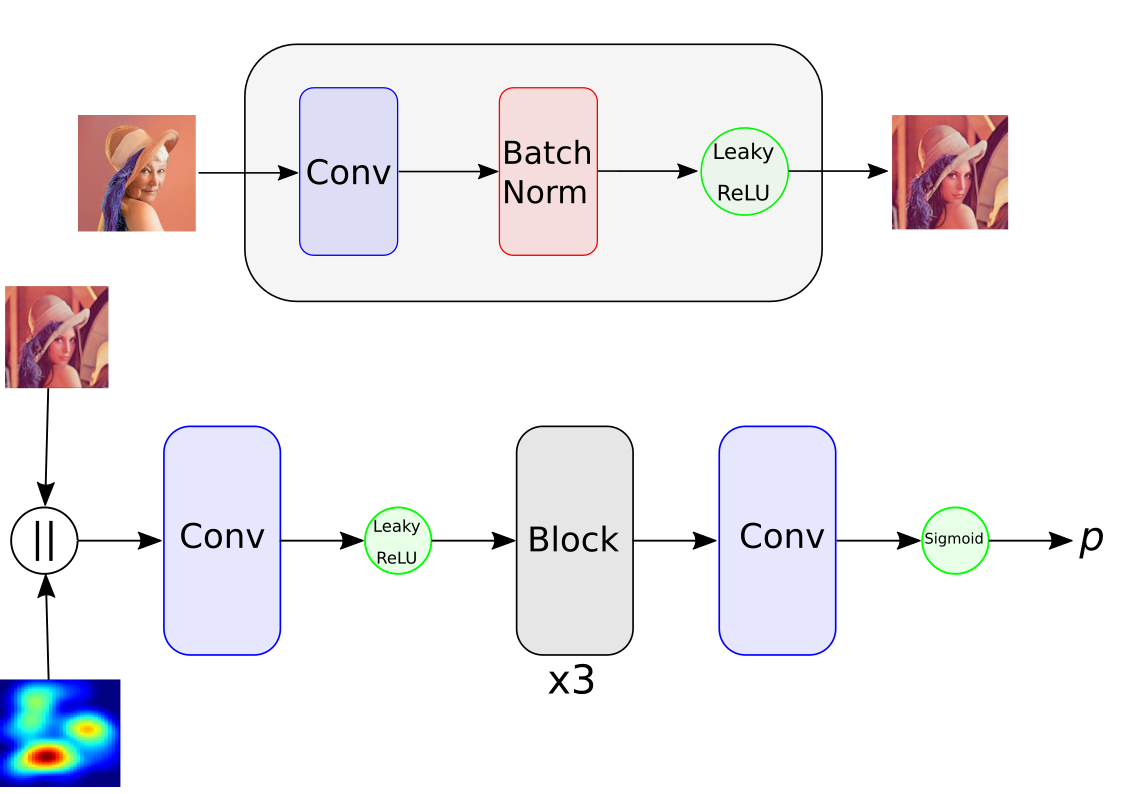
\includegraphics[scale=0.25]{images/discr.png}
   \caption{Discriminator scheme.}
   \label{fig:discriminator}
\end{figure}

\paragraph{Generator}
Generator's basic block is similiar to discriminator's one, yet instead of a convolution we employ transpose convolution to upsample, and we use ReLU as activation function.
The model is in a way simpler than the previous one:
\begin{enumerate}
   \item A sampled noise matrix is concatenated to its conditioning.
   \item We repeat generator's basic block 4 times.
   \item The model ends with a transpose convolution and a $\tanh$ activation function.
\end{enumerate}
The model is shown in figure \ref{fig:generator}, code is available on the code linked in the abstract.

\begin{figure}[h!t]
   \centering
   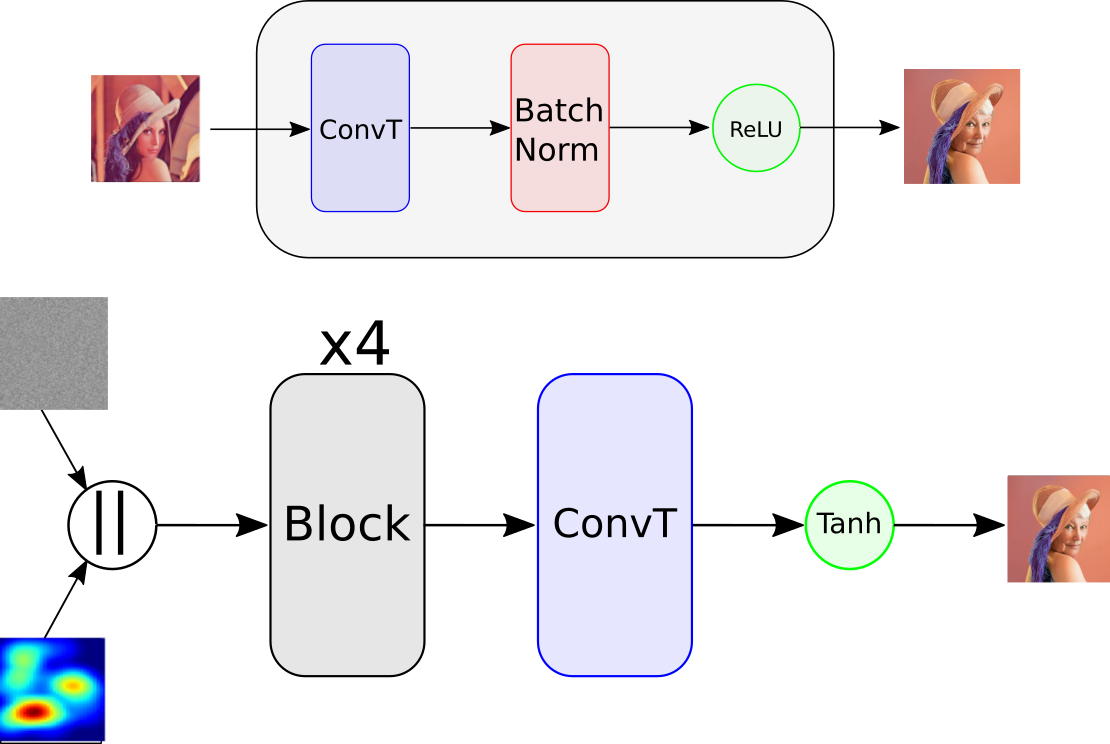
\includegraphics[scale=0.25]{images/gen.png}
   \caption{Generator scheme.}
   \label{fig:generator}
\end{figure}

\subsection{Loss}
In their seminal paper ~\cite{goodfellow2014generative}, GAN's loss is defined as a minmax loss (\ref{eq:minmax}), where $p_d$ and $p_z$ represent the distribution over real and fake data respectively.
This is quite incovenient and in the same paper it is approximated to a easier loss.
\begin{equation}
   \label{eq:minmax}
   \min_\gamma \max_\delta \mathbb{E}_{p_d} \log D(x) + \mathbb{E}_{p_z} \log (1-D(G(z)))
\end{equation}

Another approach consists in using a classical binary cross entropy loss, one each for discriminator and generator.
Discriminator's ground truth is a $\vec{0}$ for fake data and a $\vec{1}$ vector for real data, the generator's has a $\vec{1}$ too.
The generator would maximize on fake data i.e. $\vec{0}$ yet it is easier to minimize thus we flip zeros with ones.

\section{Experiments and results}
For the MNIST and FashionMNIST datasets the network has been trained for 5 and 10 epochs respectively with a learning rate equal to $0.0002$ and results are overall good.
The same cannot be said for CIFAR10, trained for 25 epochs with $0.0002$ and $0.00002$ learning rates for discriminator and generator respectively, while we can see some familiar and sensible shapes images are not realistic at all.
This makes sense since CIFAR10 scenes are way more complicated than MNIST and FashionMNIST, also having 3 channels instead of 1 could make things harder for the model.

\paragraph{Weighting}
Weighting the conditioning can give us interesting results, on the MNIST and FashionMNIST it enhances contrast and since images are black and white it means clearer outputs.

\paragraph{Multiclass conditioning}
Conditioning does not necessarily have to be a one hot vector, if more indices are equal to 1 the generator will morph images from more classes.
We can assing values different from one, even decimal, depending on what we want to create and with which strength.

\begin{figure}[h!t]
   \centering
   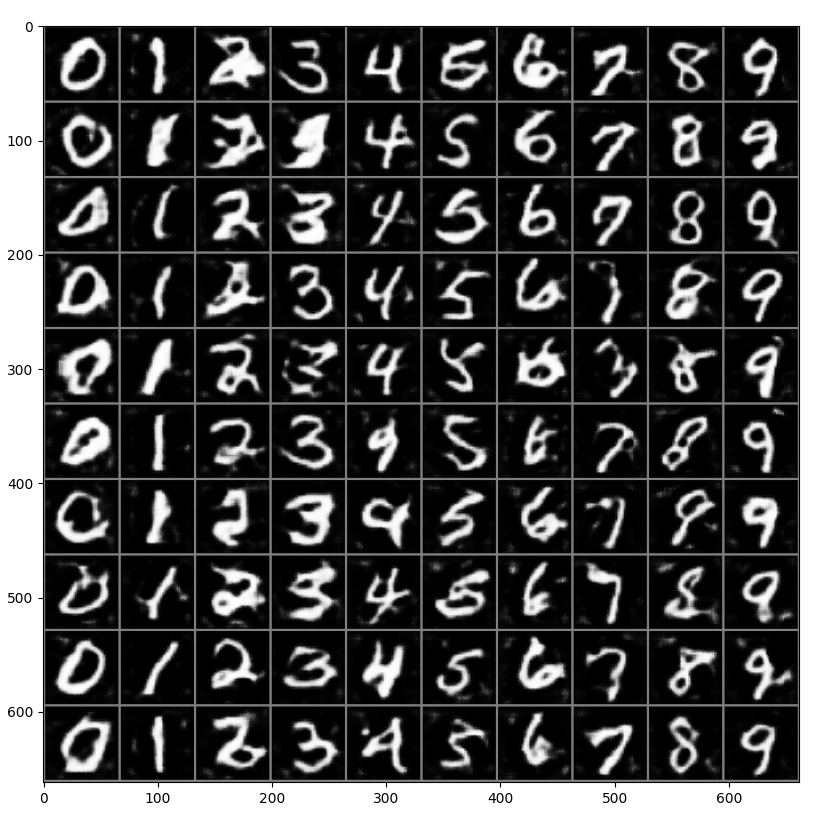
\includegraphics[scale=0.4]{images/mnist.png}
   \caption{MNIST generated images.}
   \label{fig:mnist}
\end{figure}

\begin{figure}[h!t]
   \centering
   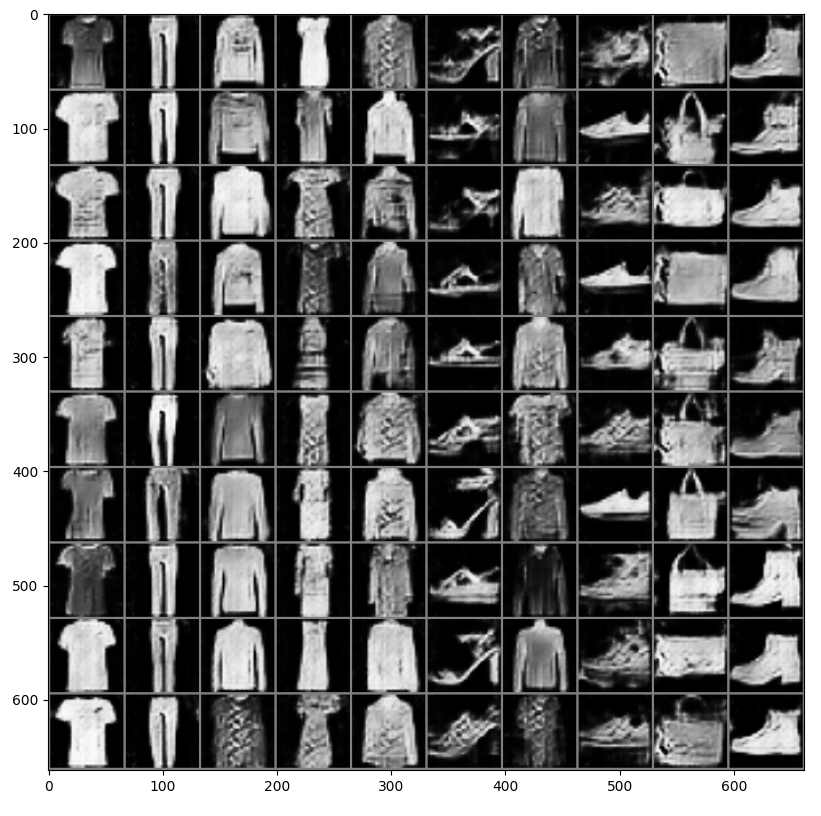
\includegraphics[scale=0.4]{images/fashion.png}
   \caption{FashionMNIST generated images.}
   \label{fig:fashion}
\end{figure}

\begin{figure}[h!t]
   \centering
   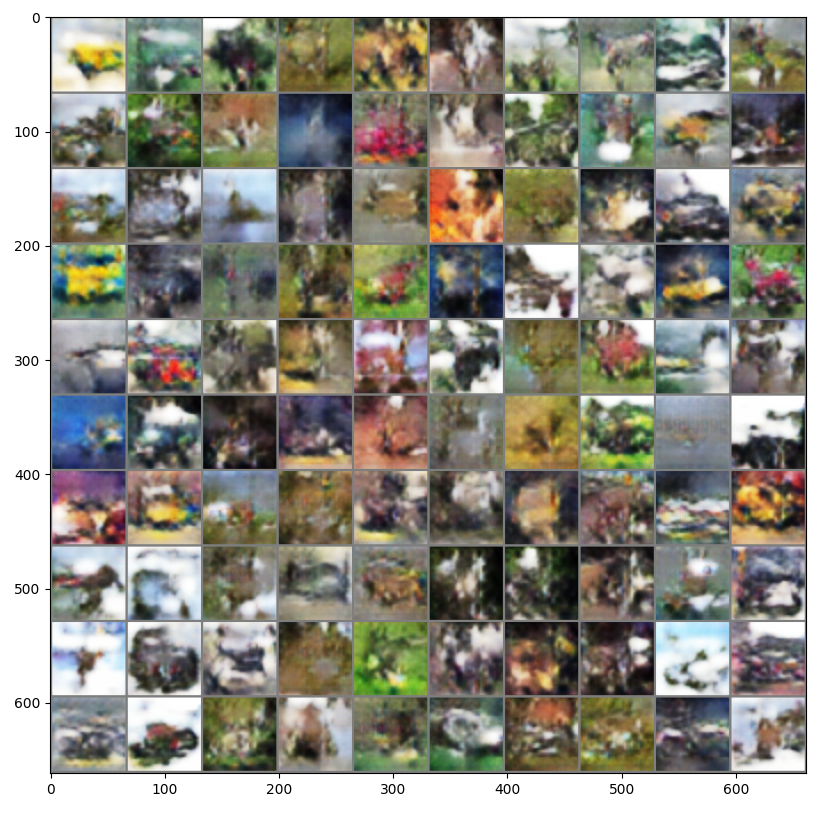
\includegraphics[scale=0.39]{images/cifar.png}
   \caption{CIFAR10 generated images.}
   \label{fig:cifar}
\end{figure}

\begin{figure}[h!t]
   \centering
   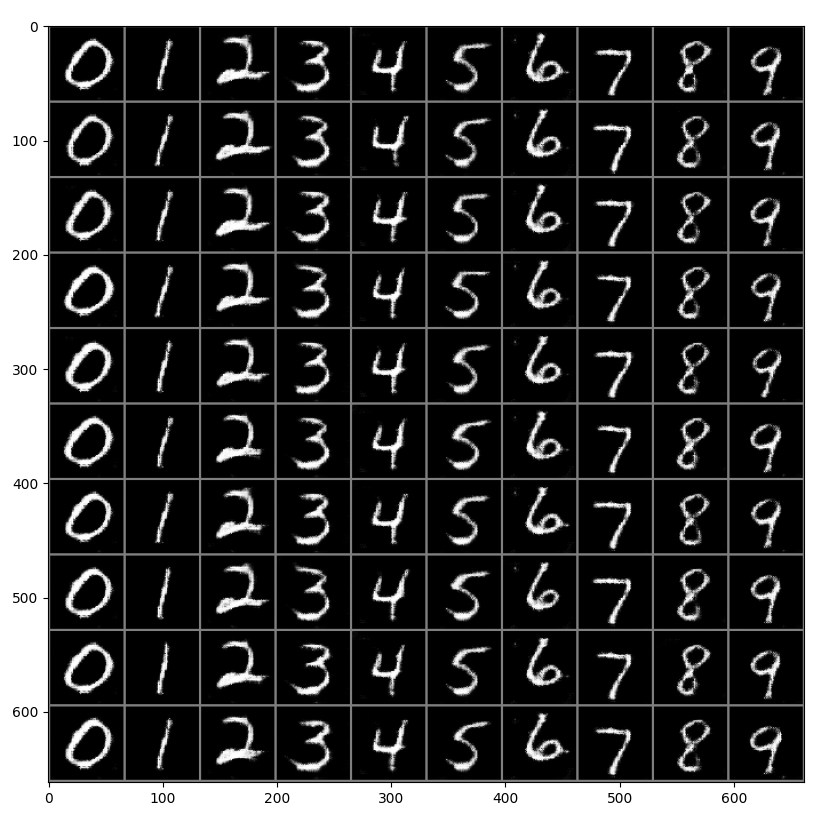
\includegraphics[scale=0.39]{images/mnist-weighted.png}
   \caption{MNIST predictions with weighted conditioning vector.}
   \label{fig:mnist-weight}
\end{figure}

\begin{figure}[h!t]
   \centering
   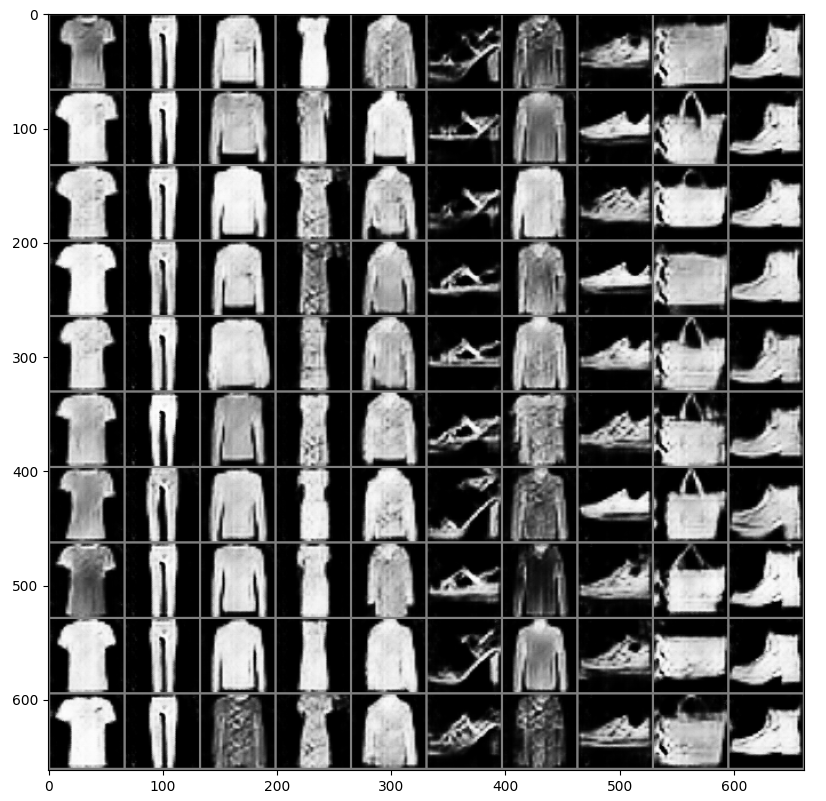
\includegraphics[scale=0.39]{images/fashion-weighted.png}
   \caption{FashionMNIST predictions with weighted conditioning vector.}
   \label{fig:fashion-weight}
\end{figure}

\begin{figure}[h!t]
   \centering
   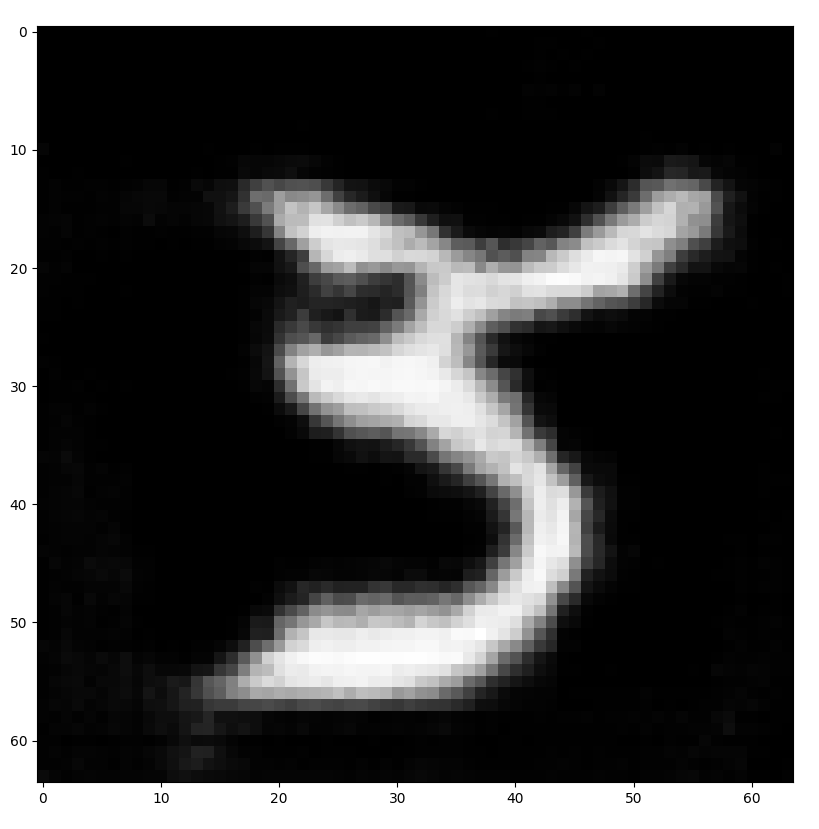
\includegraphics[scale=0.39]{images/gen35.png}
   \caption{MNIST prediction of both $3$ and $5$.}
   \label{fig:mnist-35}
\end{figure}

\begin{figure}[h!t]
   \centering
   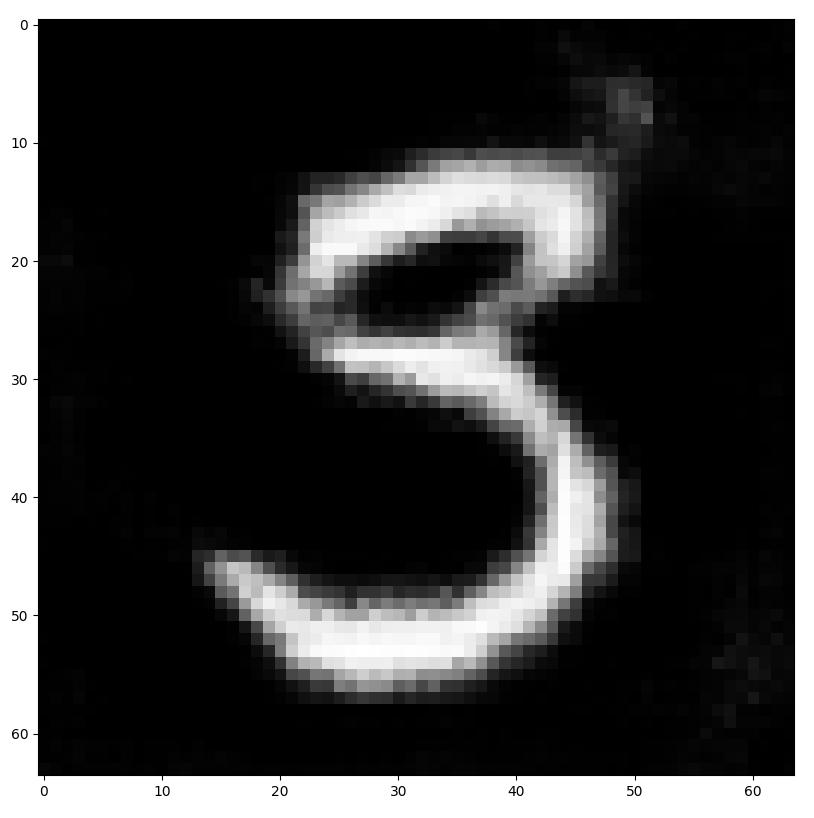
\includegraphics[scale=0.39]{images/gen35with3weighted.png}
   \caption{MNIST prediction of both $3$ and $5$, with $3$ being weighted more.}
   \label{fig:mnist-3w5}
\end{figure}

\begin{figure}[h!t]
   \centering
   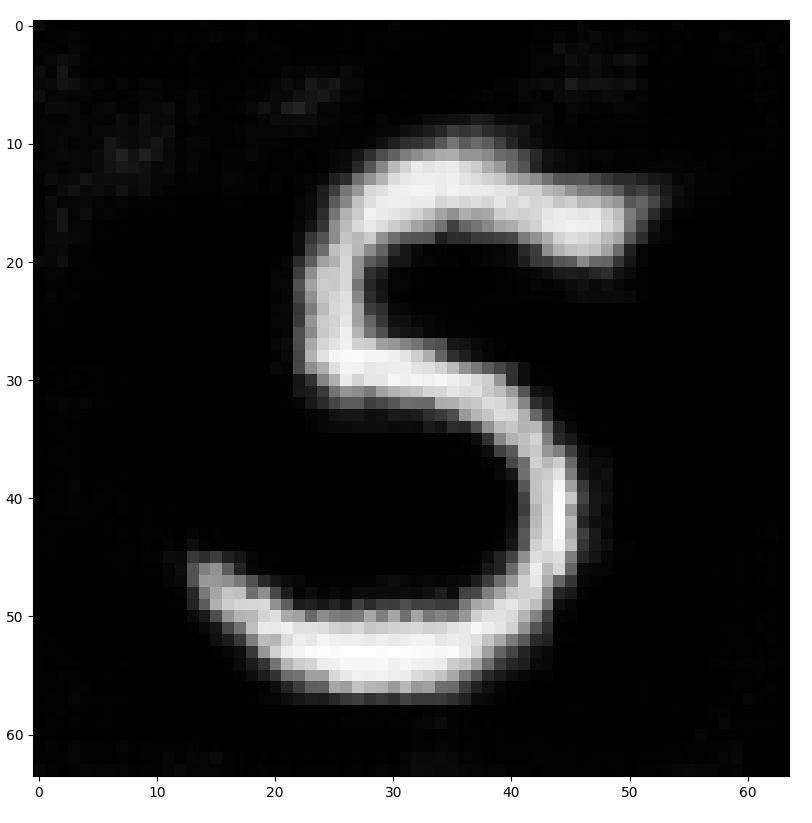
\includegraphics[scale=0.39]{images/gen35with5weighted.png}
   \caption{MNIST prediction of both $3$ and $5$, with $5$ being weighted more.}
   \label{fig:mnist-35w}
\end{figure}

\begin{figure}[h!t]
   \centering
   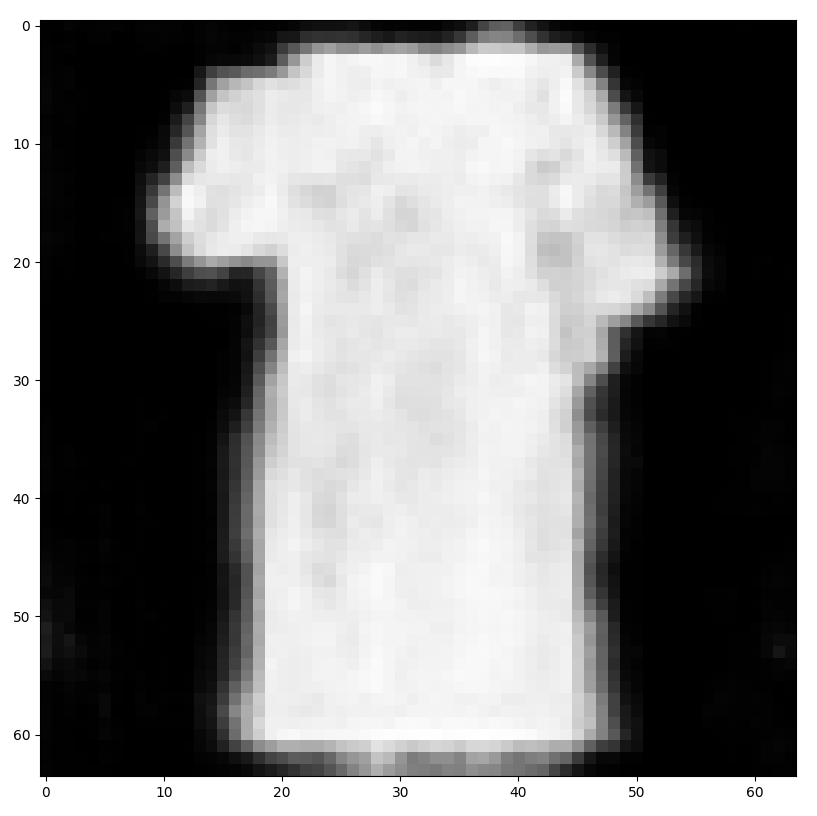
\includegraphics[scale=0.39]{images/shirt.png}
   \caption{FashionMNIST prediction of a shirt.}
   \label{fig:fashion-shirt}
\end{figure}

\begin{figure}[h!t]
   \centering
   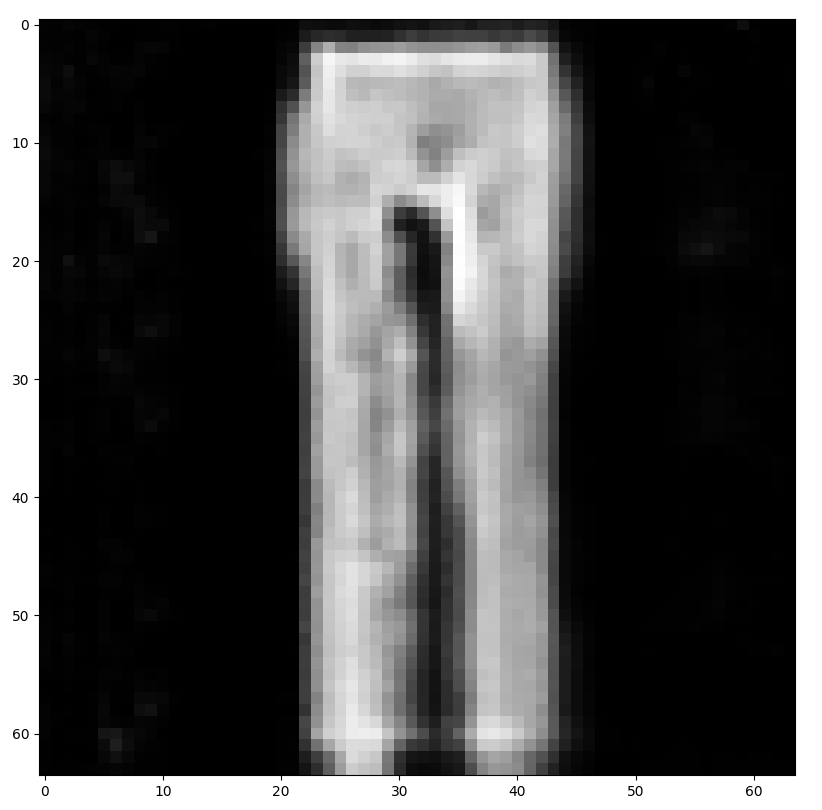
\includegraphics[scale=0.39]{images/pants.png}
   \caption{FashionMNIST prediction of a pair of pants.}
   \label{fig:fashion-pants}
\end{figure}

\begin{figure}[h!t]
   \centering
   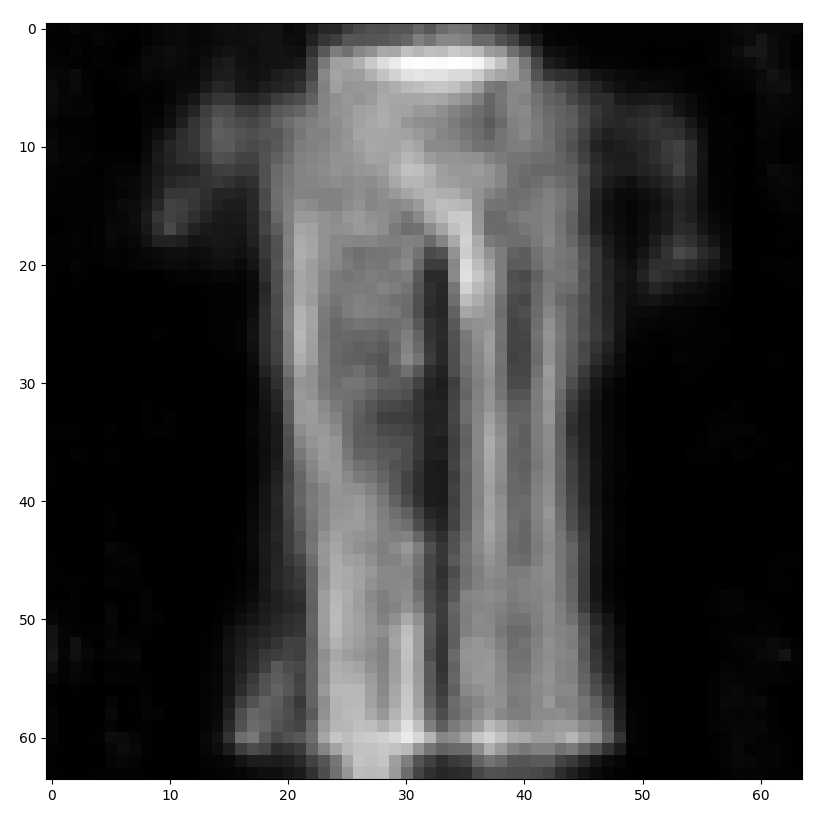
\includegraphics[scale=0.39]{images/shirtpants-weighted.png}
   \caption{FashionMNIST prediction of both shirt and pants, in this example pants are weighted $0.7$ otherwise they tend to hog the scene.}
   \label{fig:fashion-shirt-pants}
\end{figure}

\section{Conclusions}
I developed a conditional GAN that exploits convolutions, considering the relatively short training time it is quite good on simple datasets.
If the datasets gets a little more complicated results do not stand out, a plausible reason is that training GANs, other than being notoriously hard, requires large computations.

\paragraph{Future works} For this project I only had the free GPUs offered by \textit{Google Colab}, it would be interesting to see how the model does when trained properly.
Another interesting approach could be to plug in classification pretrained models as a feature extraction backbone and fine tune them.


   {\small
      \bibliographystyle{ieee}
      \bibliography{egbib}
   }

\end{document}
